% !TEX root = ../../intersection_theory.tex

\newpage
%CHAPTER 1: RATIONAL EQUIVALENCE
\section{Chapter 1: Rational Equivalence}
\subsection{Notation and Conventions}


We denote by $\A^n$ affine $n$-space and $\P^n$ projective $n$-space. For this course, by `scheme' we shall mean an algebraic scheme\footnote{Recall an affine scheme is a locally ringed space isomorphic to $\spec R$ for some commutative ring $R$ and a scheme is a locally ringed space $X$ admitting a covering by open sets $\{U_\alpha\}$ such that the restriction of the structure sheaf $\co_X$ to each $U_i$ is an affine scheme.}\footnote{An algebraic $k$-scheme is a scheme $X$ over $k$ such that the structure morphism $X \to \spec k$ is of finite type} over a field. Recall a scheme over a field is a scheme $X$ together with a morphism $p: X \to \spec k$, where $k$ is a field, and maps `backwards' on rings: for every open $U \subset X$, $\co_X(U)$ is a $k$-algebra and if $V \subset U \subset X$ are open, the restriction morphism $\co_X(U) \to \co_X(V)$ will be a $k$-algebra homomorphism. All the $\spec A_i$'s that cover $X$ will have $A_i$ as a $k$-algebra and all local rings are $k$-algebras. Note that in his text, when Fulton says \emph{algebraic}, he means the morphism is of finite type.


\begin{dfn}[Locally Finite Type]
A morphism $f: X \to Y$ is locally of finite type if there exists a covering of $Y$ by open affine subsets $V_i= \spec B_i$ such that for each $i$, $f^{-1}(V_i)$ can be covered by open affine subsets $U_{i_j} = \spec A_{ij}$, where $A_{ij}$ is a finitely generated $B_i$-algebra. 
\end{dfn}


\begin{dfn}[Finite Type]
A morphism $f: X \to Y$ is of finite type if it is of locally finite type and each $f^{-1}(V_i)$ can be covered by a finite number of the $U_{i_j}$. 
\end{dfn}


One can show (for both definitions) that if there is one affine open cover of $Y$ with the above properties then all affine open covers of $Y$ have the above properties. In our case since $\spec k$ is a single point, $X$ must have a finite affine open cover $\spec A_i$, where each $A_i$ is a finitely generated $k$-algebra. Getting rid of this assumption is important for applications of Intersection Theory to Number Theory (schemes over $\Z$). 


A variety will be reduced and irreducible scheme and a subvariety of a scheme will be a closed subscheme which is a variety. A point on a scheme will always be a closed point. 


\begin{dfn}[Connected/Irreducible]
A scheme is connected if its topology is connected. A scheme is irreducible if its topological space is irreducible. 
\end{dfn}


\begin{dfn}[Reduced]
A scheme $X$ is reduced if every open set $U$, the ring $\co_X(U)$ has no nonzero nilpotent elements; that is, if $\co_X(U)$ is a reduced ring. Equivalently, $X$ is reduced if every local ring $\co_{X,x}$ is reduced. Here, $x \in X$ need not be a closed point. 
\end{dfn}


Recall also that if $X \subset \A^n$ was an affine closed set, then $I(X)$ was a radical ideal and $A(X)=k[x_1,\ldots,x_n]/I(X)$ had no nonzero nilpotent elements. 


\begin{dfn}[Integral]
A scheme $X$ is integral if every open set $U \subseteq X$, the ring $\co_X(U)$ is an integral domain. 
\end{dfn}


\begin{prop}
A scheme is integral if and only if it is both reduced and irreducible. 
\end{prop}


This is sort of the generalization of the following fact to schemes: if $X$ is irreducible, then $I(X)$ is prime so that $A(X)=k[x_1,\ldots,x_n]/I(X)$ is an integral domain. 


\begin{dfn}[Closed Subscheme]
A closed subscheme of a scheme $X$ is a scheme $Y$ together with a morphism $i: Y \to X$ such that $\spc(Y)$ is a closed subset of $\spc(X)$, where $\spc$ is the forgetful functor to topological spaces, $i$ is the inclusion map (on the level of sets), and furthermore the induced map $i^\#: \co_X \to i_* \co_Y$ on sheaves is surjective. 
\end{dfn}


Now in the affine case, if $Y \subset X$, then $I(Y) \supset I(X)$ and $A(X)=k[x_1,\ldots,x_n]/I(X) \twoheadrightarrow k[x_1,\ldots,x_n]/I(Y)=A(Y)$. The local ring of a scheme $X$ along a subvariety $V$ is denoted $\co_{V,X}$, its maximal ideal $M_{V,X}$. [Take any affine open subset $U \subset X$ with $U \cap V \neq \emptyset$. Now $U=\spec A$ and $U \cap V$ corresponds to a prime ideal of $p \subset A$. Now $\co_{V,X}= A_p$ and check that this is independent of the choice of $U$.] The field of rational functions on a variety $X$ is denoted $R(X)$. The nonzero elements of the field $R(X)^*$ form a multiplicative group. [Take any affine open subset $U \subset X$ then $U=\spec A$. Since $X$ is a variety, $A$ will be an integral domain. Then $A=\co_X(U)$ and $R(X)=\Frac A$. Check that this is independent of the choice of $U$.]


\begin{ex}
If $f(x,y)$ and $g(x,y)$ are polynomials defining affine plane curves $F$ and $G$ over an algebraically closed field $k$, the intersection scheme $Z$ is the subscheme of $\A^2$ defined by the ideal $(f,g)$ in $k[x,y]$ generated by $f$ and $g$. If $P=(a,b)$ is a point in the plane, the intersection multiplicity of $F$ and $G$ at $P$ is defined to be $i(P,F \cdot G)=\dim_k \co_{P,Z}=\dim_k \co_{P,\A^2}/(f,g)$. The intersection multiplicity satisfies the following properties:
	\begin{enumerate}[(i)]
	\item $i(P, G\cdot F) = i(P, F \cdot G)$
	\item $i(P,(F_1+F_2)\cdot G)=i(P,F_1 \cdot G)+i(P,F_2 \cdot G)$, where $F_1+F_2$ is the ideal generated by $f_1f_2$ with $f_i$ defining $F_i$. 
	\item $i(P, F' \cdot G) = i(P, F \cdot G)$ if $F'$ is defined by $f+gh$ for some $h \in k[x,y]$ and $(f,g)=(f+gh,g)$
	\item $i(P,F \cdot G)=0$ if $P \notin F \cap G$, i.e. $P \notin F$ or $P \notin G$, and $i(P, F\cdot G)=\infty$ if $F$ and $G$ have a common component through $P$. Otherwise, $i(P, F \cdot G)$ is finite and positive. 
	\item $i(P,F \cdot G)=1$ if $f=x-a$, $g=y-b$ or generally the Jacobian $\frac{\partial(f,g)}{\partial(x,y)}$ is not zero at $P$.
	\item $i(P, G \cdot H) \geq \min\{i(P, F\cdot G), i(P, F\cdot H))$ if $P$ is a simple point of $F$ and $F$ has no common component with $G$ or $H$ through $P$.
	%picture here
	\end{enumerate}
\end{ex}


%Orders of Zeros and Poles
\subsection{Orders of Zeros and Poles}


Let $X$ be a variety and $V$ a subvariety of $X$ of dimension 1. The local ring $A=\co_{V,X}$ is a one dimensional local domain. Let $r \in R(X)^*$. We will define the order of vanishing of $r$ along $V$, $\ord_V(r)$ which will be a homomorphism: $\ord_V(rs)=\ord_V(r)+\ord_V(s)$. Any $r \in R(X)^*$ may be written as a ratio $a/b$ for $a,b \in A$. If $\ord$ is to be a homomorphism, we must define $\ord_V(r)=\ord_V(a)-\ord_V(b)$. Therefore, we must define $\ord_V(r)$ for $r \in A$. The general definition shall be 
	\[
	\ord_V(r):= l_A(A/(r))
	\]
where $l$ is the length of the module. For a fixed $r \in R(X)^*$, there are only finitely many codimension one subvarieties $V$ of $X$ with $\ord_V(r) \neq 0$. 


%Cycles and Rational Equivalence
\subsection{Cycles and Rational Equivalence}


Let $X$ be an algebraic scheme. A $k$-cycle on $X$ is a finite formal sum $\sum n_i [V_i]$, where the $V_i$ are $k$-dimensional subvarieties of $X$ and the $n_i$ are integers. The group of $k$-cycles on $X$, denoted $Z_kX$, is the free abelian group on the $k$-dimensional subvarieties of $X$; to a subvariety $V$ of $X$ corresponds to $[V]$ in $Z_kX$.


For any $(k+1)$-dimensional subvariety $W$ of $X$, and any $r \in R(W)^*$, define a $k$-cycle $[\div(r)]$ on $X$ by $[\div(r)]:=\sum \ord_V(r)[V]$, the sum over all codimension one subvarieties $V$ of $W$; this is actually a finite sum so it is an element of $Z_kX$. A $k$-cycle $\alpha \in Z_kX$ is rationally equivalent to 0, written $\alpha \sim 0$, if there are a finite number of $(k+1)$-dimensional subvarieties $W_i$ of $X$ and $r_i \in R(W_i)^*$ such that $\alpha=\sum \,[\div(r_i)]$. Since $[\div(r^{-1})]= -[\div(r)]$, the cycles rationally equivalent to 0 form a subgroup $\Rat_k X$ of $Z_kX$. Define $A_k X:= Z_kX/\Rat_kX$, $A_*= \bigoplus_{i=0}^{\dim X}$, $Z_*X= \bigoplus_{i=0}^{\dim X} Z_kX$.


\begin{dfn}[Chow Group]
The group $A_k:= Z_kX/\Rat_k X$ is called the Chow group. 
\end{dfn}


If $\alpha \in A_*X$ or $Z_kX$, $\{\alpha\}_k$ is its component in $A_k$ or $Z_k$. A cycle is positive if it is not zero and each coefficient is a positive integer. The elements of $Z_k$ are called cycles and the elements of $A_kX$ cycle classes. A cycle class is positive if it can be represented by a positive cycle. 


\begin{ex}\label{ex:1.3.2} \hfill
\begin{enumerate}[(a)]
\item A scheme and its underlying reduced scheme have the same subvarieties and therefore the groups of cycles and rational equivalence classes are canonically isomorphic:
	\[
	A_k(X)= A_k(X_\red)
	\]
Recall that if $(X,\co_X)$ is a scheme and $(\co_X)_\red$ is the sheaf associated to the presheaf $u \mapsto \co_X(U)_\red$, where for any ring $A$, we denote by $A_\red$ the quotient of $A$ by its ideal of nilpotent elements, $(X,(\co_X)_\red)$ is a scheme. We call this the reduced scheme associated to $X$ and denote it by $X_\red$. Given a irreducible closed subset $Y$ of a scheme $X$, there is one and only one structure sheaf to put on it to make it a subvariety---namely $Y_\red$.

\item If $X$ is $n$-dimensional $A_nX=Z_nX$, the free abelian group on the $n$-dimensional irreducible components of $X$. 
\end{enumerate}
\end{ex}

\begin{prop}
If $k$ is an algebraically closed field, $A_1 \A_k^1=A_1 \P_l^1=\Z$, $A_0\A_k^1=0$, $A_0 \P_k^1=\Z$.
\end{prop}

\pf The fact that $A_1 \A_k^1=A_1 \P_l^1=\Z$ follows from Example~\ref{ex:1.3.2}. For $A_0 \A_k^1=0$, we show $\Rat_1 \A_k^1=Z_1 \A_k^1$. Let $\alpha= \sum_{i=1}^s n_i [P_i]$. We have $\A_k^1=k$, $P_i=a_i \in k$. If $f=\prod_{i=1}^s (x - a_i)^{n_i}$ so $\div f= \alpha$. Now $A_0\P_k^1=\Z$ and say $\alpha= \sum_{i=1}^s n_i[P_i]$. Define $\deg \alpha = \sum_{i=1}^s n_i$. Say that $P_i=[a_i,b_i]$. If $\deg \alpha=0$ and set $f= \prod_{i=1}^s (b_ix_0 - a_ix_1)^{n_i}$ is a rational function as $\sum_{i=1}^s n_i=0$. Clearly, $\div f=\alpha$. So any degree 0 cycle is the divisor of a rational function. Since the field is algebraically closed, any polynomial factors into linear factors. Hence, any rational function's divisor will be of degree 0. Therefore, all cycles of the same degree are rationally equivalent to each other: if $\deg \alpha = \deg \beta$, then $\deg(\alpha-\beta)=0$ so $\alpha - \beta= \div f$ and $\alpha \sim \beta$. As divisors of every degree exist, $A_0 \P_k^1=\Z$. \qed \\


%Push-forward of Cycles
\subsection{Fiber Products and Separated Schemes}

Let $f: X \to Y$ be a proper morphism. 

\begin{dfn}[Fiber Product]
Let $S$ be a scheme and let $X$ and $Y$ be schemes over $S$, i.e. schemes with morphisms to $S$. We define the fibered product of $X$ and $Y$ over $S$, denoted $X \times_S Y$ to be a scheme together with morphisms $p_1: X \times_S Y \to X$ and $p_2: X \times_S Y \to Y$ which make a commutative diagram with the given morphisms $X \to S$ and $Y \to S$
	\[
	\begin{tikzcd}
	Z \arrow[yshift=1ex]{drr}{g} \arrow[dotted,swap]{dr}{\theta} \arrow[swap,xshift=-1.5ex]{ddr}{f} & & \\
	& X \times_S Y \arrow{r}{p_2} \arrow[swap]{d}{p_1} & Y \arrow{d}{q_2} \\
	& X \arrow[swap]{r}{q_1} & S
	\end{tikzcd}
	\]
such that given any scheme $Z$ over $S$ and given morphisms $f: Z \to X$ and $g: Z \to Y$ which makes the given morphisms $X \to S$ and $Y \to S$, then there is a unique morphism $\theta: Z \to X \times_S Y$ such that $f=p_1 \theta$ and $g= p_2 \theta$. Set theoretically, $\theta(p)=(f(p),g(p))$, $X \times_S Y=\{(x,y) \colon q_1p_1(x,y)=q_2p_2(x,y)\}$. The morphisms $p_1$ and $p_2$ are called the projection morphisms of the fibered product onto its factors. If $X$ and $Y$ are schemes given without reference to any base scheme $S$, we take $S=\spec \Z$ and define the product of $X$ and $Y$ to be $X \times_{\spec \Z} Y$.
\end{dfn}


\begin{exc}
Describe $\spec \Z$ and show that it is a final object for the category of schemes, i.e. each scheme $X$ admits a unique morphism to $\spec \Z$. 
\end{exc}


\begin{thmm}
For any two schemes $X$ and $Y$ over a scheme $S$, the fibered product exists and is unique up to isomorphism. 
\end{thmm}

\pf The idea of the proof is that 
	\[
	\begin{tikzcd}
	C \arrow{r}{\varphi} \arrow[swap]{d}{\psi} & B \arrow[swap]{d}{\beta} \arrow[yshift=1ex]{ddr}{\beta'} &  \\
	A \arrow{r}{\alpha} \arrow[swap,yshift=-1ex]{drr}{\alpha'} & A \otimes_C B \arrow[dotted]{dr}{\theta} &  \\
	 &  & Z \\
	\end{tikzcd}
	\]
is the desired universal diagram with arrows reversed. Taking $\spec$ of everything gives the desired diagram. It is then a matter of checking that everything glues together nicely. 


\begin{dfn}[Separated Scheme]
Let $f: X \to Y$ be a morphism of schemes. The diagonal morphism is the unique morphism $\Delta: X \to X \times_Y X$ whose composition with both projection morphisms $p_1,p_2: X \times_Y X \to X$ is the identity map of $X \to X$. We say that the morphism $f$ is separated if the diagonal morphism $\Delta$ is a closed immersion. In that case, we say that $X$ is separated over $Y$. A scheme $X$ is separated if it is separated over $\spec \Z$. 
\end{dfn}

To show that such a $\Delta$ exists, first work with affine schemes and tensor products. 
	\[
	\begin{tikzcd}
	A  \arrow{dr}{a \mapsto a \otimes 1} & & \\
	& A \otimes_B A \arrow{r}{a_1 \otimes a_2 \mapsto a_1a_2} & \;\;\;A \\
	A \arrow[swap]{ur}{a \mapsto 1 \otimes a} & & 
	\end{tikzcd}
	\]
Now when Hartshorne says immersion, he means an embedding (imbedding). So self crossings as in the diagram below is allowed in differential geometry but not in the sense of Hartshorne's algebraic geometry.  
% ) \to \alpha
We say $f: X \to Y$ is a closed (open) immersion if $f$ induces an isomorphism onto a closed (open) subscheme of $Y$. 

\begin{dfn}[(Locally) Noetherian]
A scheme $X$ is locally noetherian if it can be covered by open affine subsets $\spec A_i$, where each $A_i$ is a noetherian ring. A scheme $X$ is noetherian if it is locally noetherian and quasi-compact. Equivalently, $X$ is noetherian if it can be covered by a finite number of open affine subsets $\spec A_i$ with each $A_i$ a noetherian ring. 
\end{dfn}

\begin{rem}
If $X$ is a noetherian scheme then $\text{sp}(X)$ is a noetherian topological space but not conversely. 
\end{rem}

\begin{dfn}
Let $F$ be a field and $D \subset F$ a subintegral domain. $D$ is said to be a valuation ring for $F$ if and only if for all $x \in F$, either $x \in D$ or $x^{-1} \in D$.
\end{dfn}

\begin{ex}
Let $p \in \Z$ be a prime number. Then $(p)$ is the prime ideal $p\Z$. Then $\Z_{(p)}$ is a valuation ring. Write $a/b$ in lowest terms then either $p\nmid a$ or $p \nmid b$. It is easy to see that if $D$ is a valuation ring for $F$ then $F=\Frac D$. A bit harder to show is that $D$ is a local ring. 
\end{ex}

\begin{ex}
$\Z \subseteq \Q$ is not a valuation ring as $2/3 \notin \Z$ and $3/2 \notin \Z$.
\end{ex}


\begin{prop}[Valuative Criterion of Separatedness]
Let $f: X \to Y$ be a morphism of schemes and assume $X$ is noetherian. Then $f$ is separated if and only if for any field $K$ and for any valuation ring with quotient field $K$, letting $T=\spec R$, $U=\spec K$, and $i: U \to T$ be the morphism induced by the inclusion $R \subseteq K$, given a morphism of $T$ to $Y$ and a morphism from $U$ to $X$ that gives a commutative diagram
	\[
	\begin{tikzcd}
	U \arrow{d} \arrow{r} & X \arrow{d}{f} \\
	T \arrow[dotted]{ur} \arrow{r} & Y 
	\end{tikzcd}
	\]
there is at most one morphism of $T$ to $X$ making the whole diagram commute. 
\end{prop}


\noindent Now the $\spec$ map pulled back primes and $U=\spec k$ is one-point. Now $j: R \to k$ is an injection so that $j^{-1}(0)=(0)$ is contained in all primes so that it must be the generic point. We are trying to lift $g$ to $l: T \to X$. The diagram says $h$ is a lifting almost everywhere -- you need only complete the lifting. Separated says there is at most one way to do it. 


\begin{ex}
Start with two copies of $\A^1$ and $P \in \A^1$. Glue the two copies of $\A^1 \setminus\{P\}$ via the obvious identity map but do not glue at $\{P\}$. The new space `looks' like $\A^1$ but $P$ is doubled. Call it $X$. 
	\begin{figure}[H]
	   \centering
	   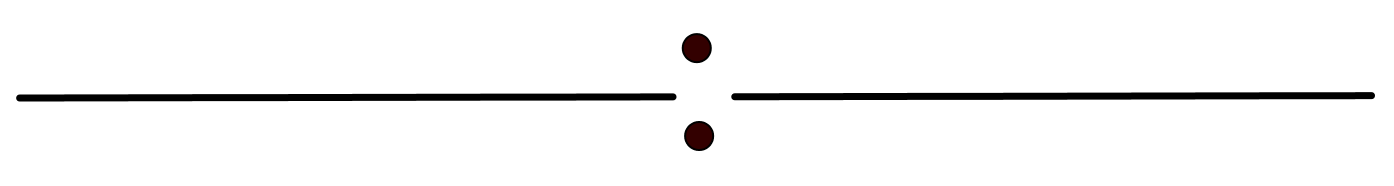
\includegraphics[width=0.4\textwidth]{doublepoint.png} 
	\end{figure}
Then this is not separated as limits, if they exist, must be unique.
	\begin{figure}[H]
	   \centering
	   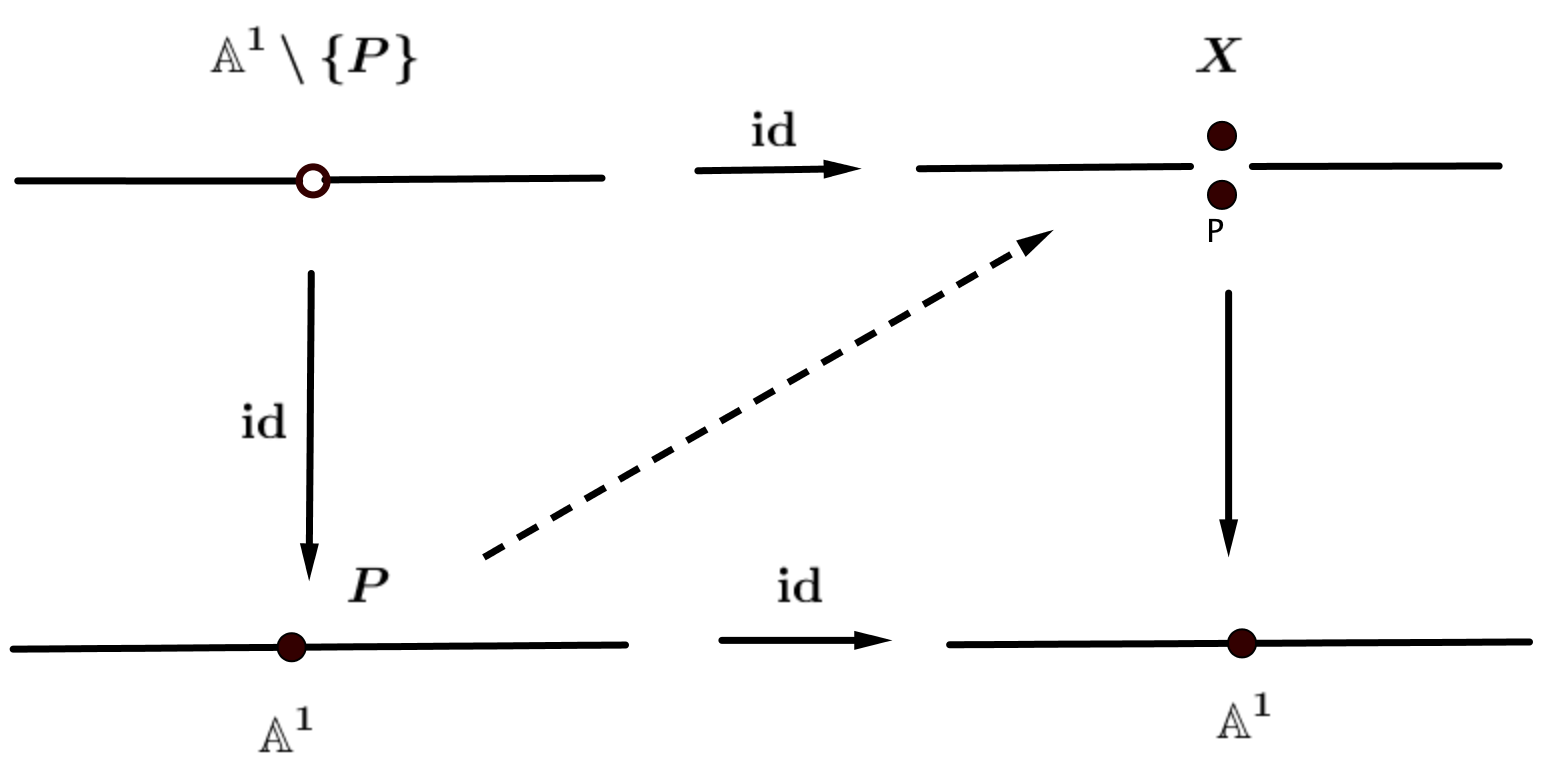
\includegraphics[width=0.5\textwidth]{doublepoint2.png} 
	\end{figure}
\end{ex}


\begin{dfn}[Stable Under Base Extension]
Let $f: X \to Y$ and $g: Y \to Y'$ be morphisms. Standard properties of the fiber product give a morphism $p_2: X \times_Y \to Y'$. Often, one denotes $p_2$ by $f'$ and $X \times_Y Y'$ by $X'$ and say $f': X' \to Y'$ is obtained from $f: X \to Y$ by base extension (change). Let $S$ be any property of a morphism. We say that $S$ is stable under base extension if and only if $f$ has $S$, then $f'$ has $S$.
\end{dfn}


\begin{prop}
Assume that the underlying schemes are noetherian:
\begin{enumerate}[(a)]
\item Open and closed immersions are separated.
\item A composition of two separated morphisms is separated.
\item Separated morphisms are stable under base extension.
\item If $f: X \to Y$ and $f': X' \to Y'$ are separated morphisms over a vase scheme $S$, then the product morphism $f \times f': X \times_S X' \to Y \times_S Y'$ is also separated.
\item If $f: X \to Y$ and $g: Y \to Z$ are two morphisms and $g \circ f$ is separated then $f$ is separated.
\item A morphism $f: X \to Y$ is separated if and only if $Y$ can be covered by open subsets $V_i$ such that $f^{-1}(V_i) \to V_i$ is separated for each $i$. 
\end{enumerate}
\end{prop}


\begin{dfn}[Proper Morphism]
A morphism $f: X \to Y$ is proper if it is separated, has finite type, and is universally closed. Here we say a morphism is closed if the image of any closed set is closed. A morphism $f: X \to Y$ is universally closed if it is closed and for any morphism $Y' \to Y$, the corresponding morphism $f': X' \to Y'$ obtained by base extension is also closed.
\end{dfn}


\begin{thmm}
Let $f: X \to Y$ be a morphism of finite type with $X$ noetherian. Then $f$ is proper if and only if for every valuation ring $R$ and for every morphism of $U$ to $X$ and $T$ to $Y$ forming a commutative diagram (using the notation as before), there exists a unique morphism $T \to X$ making the whole diagram commute. 
	\[
	\begin{tikzcd}
	U \arrow{d}{i} \arrow{r} & X \arrow{d}{f} \\
	T \arrow[dotted]{ur} \arrow{r} & Y 
	\end{tikzcd}
	\] 
\end{thmm}


\begin{ex}
Recall the blow-up of a point in $\A^n$
	\[
	\begin{tikzcd}
	X \arrow[hook]{r} \arrow[swap]{dr}{\phi} & \A^n \times \P^{n-1} \arrow{d} \\
	& \A^n
	\end{tikzcd}
	\]
$\phi$ is proper because it is projective. We took any line $L$ through $(0,\ldots,0)$ in $\A^n$ lifted $L \setminus \{(0,\ldots,0)\}$ to $X$ then took its closure $\tilde{L} \subset X$. $\tilde{L}$ met $\phi^{-1}((0,\ldots,0))$ at a point corresponding to the ``slopes'' of $L$, $\phi(\tilde{L})=L$.
	\begin{figure}[H]
	   \centering
	   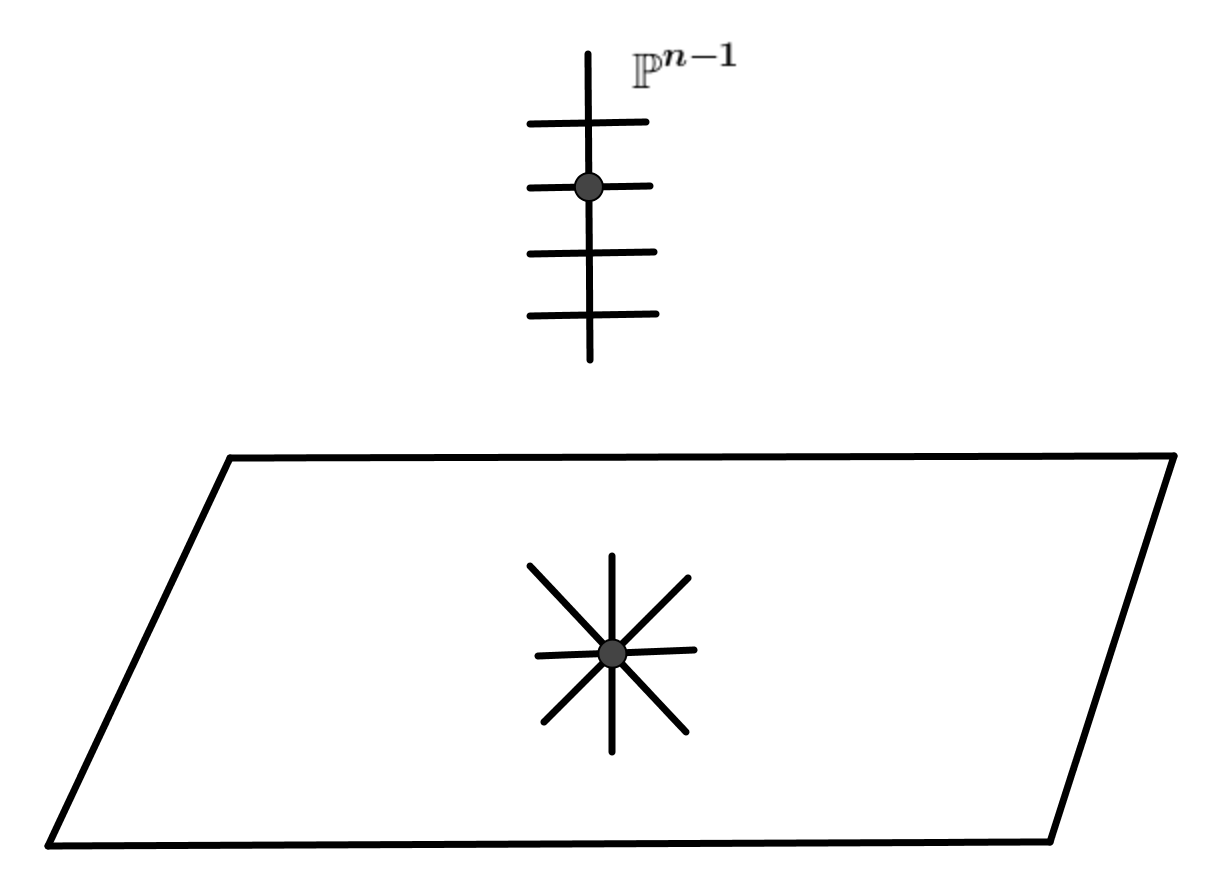
\includegraphics[width=0.5\textwidth]{projplane.png} 
	\end{figure}
If you replace $X$ by $X \setminus \{P\}$ for some $P \in \phi^{-1}((0,\ldots,0))$, it is not proper anymore. The corresponding line will not have its limit.
\end{ex}


Proper morphisms are like projective varieties. You can not get rid of something by pushing it off to $\infty$. IN $\A^2$, parallel lines do not meet because you pushed the intersection off to $\infty$. In $\P^2$, they do meet.


\begin{cor}
Assuming the underlying schemes are noetherian:
\begin{enumerate}[(a)]
\item A closed immersion is proper.
\item A composition of proper morphisms is proper.
\item Proper morphisms are stable under base extension.
\item Products of proper morphisms are proper.
\item If $f: X \to Y$ and $g: Y \to Z$ are two morphisms, $g \circ f$ is proper, and $g$ is separated then $f$ is proper.
\item Properness is local on the base.
\end{enumerate}
\end{cor}


\begin{dfn}[Projective Morphism]
If $Y$ is a scheme, we define projective $n$-space over $Y$, denoted $\P^n_Y$, to be $\P^n_\Z \times_{\spec \Z} Y$. A morphism $f: X \to Y$ of schemes is projective if it factors into a closed immersion $i: Y \hookrightarrow \P_Y^n$ for some $n$, followed by the projection $\P_Y^n \to Y$. A morphism is quasi-projective if it factors into an open immersion $j: X \to X'$ followed by a projective morphism $g: X' \to Y$. 
\end{dfn}


\begin{thmm}
A projective morphism of a noetherian scheme is proper. A quasi-projective morphism of noetherian schemes is of finite type and separated. 
\end{thmm}


Given any quasi-projective variety, you can construct the associated scheme:


\begin{prop}
Let $k$ be an algebraically closed field. The image of the functor $F: \text{Var}(k) \to \text{Sch}(k)$ (varieties over $k$ to schemes over $k$) is exactly the set of quasi-projective integral schemes of $k$. The image of the set of projective varieties is the set of projective integral schemes over $k$. In particular, for any variety $V$, $F(V)$ is an integral separated scheme of finite type over $k$. 
\end{prop}


\begin{dfn}
An abstract variety is an integral, separated scheme of finite type over an algebraically closed field $k$. If it is proper over $k$, we will also say it is complete. 
\end{dfn}


Note that complete curve is projective and every nonsingular complete surface is projective (Zariski). Finally, there exists a nonsingular complete nonprojective three-folds (Nagata, Hironata, Appendix B). But every variety can be embedded as an open dense subset of a complete variety (Nagata). So completeness is like algebra-geometric version of the analysis' compactness. 


%Pushforward of Cycles
\subsection{Push-forward of Cycles}

Let $f: X \to Y$ be a proper morphism. We want to first define $f_*: Z_k X \to Z_k Y$ and then show that $f_*(\Rat_k X) \subset \Rat_k Y$. This will give a map $f_*: A_k X \to A_k Y$ since $Z_kX$ is a free abelian group you only need to define $f_*$ on the generators. The generators are the $k$-dimensional subvarieties of $X$. Let $V$ be a $k$-dimensional subvariety of $X$. Since $f$ is proper, $f(V)$ is closed in $Y$. Continuous images of irreducible sets are irreducible and the morphisms here are continuous. Therefore, $f(V)$ is also irreducible. If the domain of a map is a reduced space, then the image is automatically reduced so $f(V)$ is a variety. Now $R(V)$ and $R(f(V))$ are both fields. Pullback of functions makes $R(f(V))$ a subfield of $R(V)$. Our assumptions on schemes, being finite type over a field, makes the relation between dimension and transcendence degrees of function fields remain valid. Then as $R(f(V)) \subset R(V)$, $\text{tr deg}_kR(f(V)) \leq \text{tr deg}_kR(V)$. But then $\dim f(V) \leq \dim V$. When $\dim f(V)=V$, this says that $R(f(V)) \subset R(V)$ is an algebraic extension of finite type over a field says that they both must be finitely generated over $k$ as finitely generated and algebraic implies finite. Then $R(f(V)) \subset R(V)$ is a finite extension and denote the degree of the extension by $[R(V):R(f(V))]$. Define
	\[
	\deg(V/f(V))=
	\begin{cases}
	[R(V):R(f(V))], & \text{if } \dim V=\dim f(V) \\
	0, \text{otherwise}
	\end{cases}
	\]
Note we cannot have $\dim f(V) > \dim V$. Let $W=f(V)$. Then we can define $f_*[V]= \deg(V/W)[W]$. This gives $f_*: Z_k X \to Z_k Y$ and if $X \ma{f} Y \ma{g} Z$, $(g \circ f)_*=g_*f_*$ because degrees of field extensions are multiplicative. If $k=\C$ or if $R(W) \subset R(V)$ is a separable extension and $k$ is algebraically closed, then $f: V \to W$ is generically a $[R(V):R(W)]$ sheeted cover. When the extension is inseparable, the cases become more pathological. When $k=\C$, this agrees with the push forward of homology in topology. 


\begin{thmm}\label{thm:ratequiv}
If $f: X \to Y$ is a proper morphism and $\alpha$ is a $k$-cycle of $X$ that is rationally equivalent to zero on $Y$, there is an induced homomorphism $f_*: A_k X \to A_k Y$ such that $A_*$ is a covariant functor for proper morphisms. 
\end{thmm}


The proof uses the fact that we may assume $\alpha=[\div r]$, where $r$ is a rational function on a subvariety of $X$. We may replace $X$ by this subvariety and replace $Y$ by $f(X)$. Therefore, we may assume $Y$ is a variety and $f$ is surjective. 


If $K \subset L$ is a finite field extension. If $a \in L$, we denote the norm of $a$ in $K$ as $N(a) \in K$. Define $f: L \to L$ by $f(x)=ax$. Now $f$ is a $k$-linear transformation. Choose a $k$-basis for $L$ and make the matrix representing the map as $M$. Define also $N(a)=\det M$. If you were to choose a different basis and get a matrix representation $M'$, $M'=PMP^{-1}$ for some invertible $P$. But then $\det(M')=\det(PMP^{-1})=\det M$, independent of the choice of basis.  


\begin{prop}
Let $f: X \to Y$ be a proper surjective morphism of varieties and let $r \in R(X)^*$. Then $f_*[\div r]=0$ if $\dim Y <\dim X$ and $f_*[\div r]=[\div(N(r))]$ if $\dim Y=\dim X$.
\end{prop}


\begin{dfn}
If $X$ is a complete scheme, i.e. $X$ is proper over $S=\Spec k$, $k$ the ground field, and $\alpha=\sum_P n_P[P]$ is a zero cycle on $X$, the degree of $\alpha$, denoted $\deg \alpha$ or $\int_X \alpha$ is defined by 
	\[
	\deg \alpha = \int_X \alpha = \sum_P n_P [R(P):k] 
	\]
Equivalently, $\deg \alpha = p_X(\alpha)$, where $p$ is the structure morphism from $X$ to $S$ and $A_0(S)=\Z[S]$ is identified with $\Z$.
	\[
	p: X \ma{\text{proper}} S=\Spec k
	\]
\end{dfn}


By Theorem~\ref{thm:ratequiv}, rationally equivalent cycles have the same degree: $\deg \div r=0$. The only way to be rationally equivalent to zero on $S=\Spec k$ is to be identically zero. We can extend the degree homomorphism to all of $A_*X$
	\[
	\int_X: A_* \to \Z
	\]
by defining $\int_X \alpha=0$ if $\alpha \in A_k X$ for $k>0$. For any morphism of complete schemes $f: X \to Y$ and any $\alpha \in A_* X$, $\int_X \alpha=\int_Y f_*(\alpha)$. Sometimes, we simply write $\int$ instead of $\int_X$. Now if $f: X \to Y$ and $g: Y \to Z$ are two morphisms, if $g \circ f$ is proper and $g$ is separated, then $f$ is proper.
	\[
	\begin{tikzcd}
	X \arrow{r}{f} \arrow{dr}{h} & Y \arrow{d}{g} \\
	& \Spec k=Z
	\end{tikzcd}
	\]
Now $X,Y$ complete say that $h,g$ are proper. Now $g \circ f=h$ is proper. But $g$ is proper and hence is separated. But then $f$ is proper. Now $\int_X \alpha=h_*\alpha$ and $\int_Y f_*(\alpha)=g_*f_*(\alpha)=h_*(\alpha)$. 


\begin{ex}
Theorem~\ref{thm:ratequiv} implies B\'ezout's Theorem for plane curves over an algebraically closed field: if $F$ and $G$ are curves of degree $m,n$ with no common components, then
	\[
	\sum_{P \in \P^2} i(P,F \cdot G) = mn
	\]
One may assume $F$ is irreducible:
	\[
	i(P,\underbrace{F_1F_2}_{F_1+F_2} \cdot G)=i(P,F_1 \cdot G)+i(P, F_2 \cdot G)
	\]
If $G$ and $G'$ have degree $n$, then $G/G'$ defines a rational function $r$ on the curve $F$ and 
	\[
	\sum i(P,F \cdot G) - \sum i(P,F \cdot G') = \sum \ord_P(r) = 0 
	\]
Assume $G$ is a product of lines. Use irreducibility to assume $G$ is a line. Then reverse the roles of $F,G$ and assume $F$ is a line. Then merely check two lines intersect at one point. 
\end{ex}


%Cycles of Subschemes
\subsection{Cycles of Subschemes}

Let $X$ be any scheme and Let $X_1,\ldots,X_t$ be the irreducible components of $X$. The local rings $\co_{X_i,X}$ are all zero-dimensional (Artinian). [The irreducible components correspond to maximal irreducible closed subsets which correspond to minimal prime ideals and when you localize you get a zero dimensional ring.] The geometric multiplicity of $X_i$ in $X$, $m_i$, are
	\[
	m_i= l_{\co_{X_i,X}} \co_{X_i,X}
	\]
The fundamental cycle $[X]$ of $X$ is the cycle $[X]=\sum_{i=1}^t m_i [X_i]$.

\begin{dfn}
If $f: X \to Y$ is a morphism and $Z$ is a subscheme of $Y$, the inverse image scheme, denoted $f^{-1}(Z)$, may be identified with the fiber product $X \times_Y Z$. 
	\[
	\begin{tikzcd}
	X \arrow[swap]{d}{f} & X \times_Y Z \arrow{l}{p_2} \arrow{d}{p_1} \\
	Y & Z \arrow[hook]{l}{i}
	\end{tikzcd}
	\]
Since $i$ is a closed embedding, $p_2$ is a closed embedding. If $I$ is the ideal sheaf of $Z$ in $Y$, then $f^{-1}(Z)$ is defined by the ideal $f^{-1}(I) \co_X$. [Note: if $U \subset Y$, then $I_Y(U) \subset \co_Y(U)$ is everything vanishing on $Y$.]
\end{dfn}

\begin{ex}
As a trivial example 
	\[
	\begin{tikzcd}
	\A^1 \arrow{r} \arrow[dash]{d} & \A^1 \arrow[dash]{d} \\
	k[x] & k[t] \arrow{l}{\phi}
	\end{tikzcd}
	\]
where $\phi(t)=x^2$.

	\begin{figure}[H]
	   \centering
	   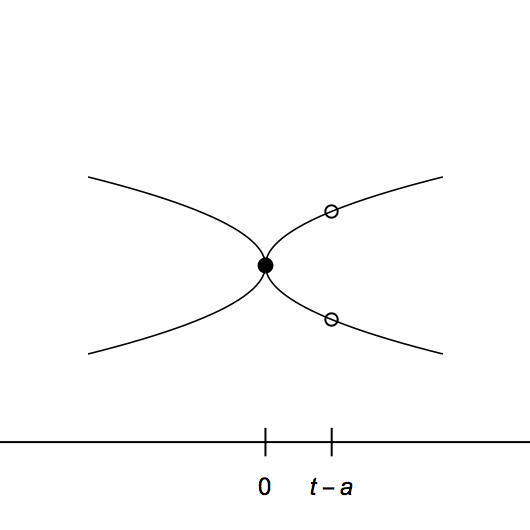
\includegraphics[width=0.5\textwidth]{parab.png} 
	\end{figure}
$x^2-a=(x-a)(x+a)$. $k[x]/(x^2)$. 	
\end{ex}

\begin{ex}
Let $V$ be a variety of dimension $k+1$ and $f: V \to \P^1$ a dominant morphism. Let $0=(1,0)$ and $\infty=(0,1)$ be the zero and infinite points of $\P^1$. The inverse image schemes $f^{-1}(0)$ and $f^{-1}(\infty)$ are purely $k$-dimensional subschemes of $V$ and the cycle $[f^{-1}(0)] - [f^{-1}(\infty)]$ correspond to the cycle $[\div f]$, where $f$ also denotes the rational function in $R(V)$ determined by the morphism $f$. $[f^{-1}(0)]$ is rationally equivalent to $[f^{-1}(\infty)]$. This is sort of like homotopy in topology where we are deforming the fiber $f^{-1}(0)$ into the fiber $f^{-1}(\infty)$. The big difference is the only 1-dimensional real manifold without boundary is $S^1$. In Algebraic Geometry, there are many 1-dimensional nonsingular projective curves. 
\end{ex}

\begin{dfn}
Two $k$-cycles $\alpha,\beta$ on $V$, a $(k+1)$-dimensional variety, are algebraically equivalent if and only if there is a dominant morphism $f: V \to Y$ where $Y$ is a nonsingular curve and two points $P,Q \in Y$ with $\alpha=[f^{-1}(P)]$, $\beta=[f^{-1}(Q)]$ rationally equivalent (hence algebraically equivalent). The converse is not true. 
\end{dfn}


%Flat Pull-back of Cycles
\subsection{Flat Pull-back of Cycles}

\begin{dfn}[Flat]
Let $f: X \to Y$ be a morphism of schemes. Let $P \in X$ be a point (closed or not) and let $Q=f(P)$. We get an induced homomorphism $f^*: \co_{Q,Y} \to \co_{P,X}$. We say that $f$ is flat at $P$ if and only if $\co_{P,X}$ is a flat $\co_{Q,Y}$ module. We say $f$ is flat if and only if it is flat at every point $P \in X$. 
\end{dfn}

Fulton gives the following (equivalent) definition:

\begin{dfn}
A morphism $f: X \to Y$ is flat if and only if for (any) $U \subset Y$, $U' \subset X$ affine open sets with $f(U') \subset U$ the induced map $f^*: A(U) \to A(U')$ makes $A(U')$ a flat $A(U)$ module. 
\end{dfn}


Recall by Algebra nonsense if $M$ is an $A$-module, then $M$ is a flat $A$-module if and only if $M_p$ is a flat $A_p$-module for all $p \in \spec A$. A morphism $f: X \to Y$ has relative dimension $n$ if and only if for all subvarieties $V$ of $Y$ and all irreducible components $V'$ of $f^{-1}(V)$, $\dim V'=\dim V+n$. If $f$ is flat, $Y$ is irreducible and $X$ has pure dimension equal to $\dim Y+n$, then $f$ has relative dimension $n$ and all base extensions $X \times_Y Y' \to Y$ have relative dimension $n$. A flat morphism is assumed to have a relative dimension. Now open immersions are flat and flatness is stable under base extensions. Compositions of flat maps are flat. 


\begin{thmm}
Let $T$ be an integral noetherian scheme. Let $X \subseteq \P^n_T$ be a closed subscheme. For each point $t \in T$, we consider the Hilbert polynomial $P_t \in \Q[z]$ of the fiber $X_t$ considered as a closed subscheme of $\P^n_{k(t)}$. Then $X$ is flat over $T$ if and only if the Hilbert polynomial is independent of $t$. 
\end{thmm}
	\[
	\begin{tikzcd}
	X \arrow[swap]{dr}{\pi} \arrow[hook]{r} & \P^n \times T \arrow{d}{p_2} \\
	& T 
	\end{tikzcd}
	\]
For $t \in T$, $p_2^{-1}(t)=\P^n$, $\pi^{-1}(t)= \P^n \cap X$ which is some closed subscheme of $\P^n$. This is a varying family of closed subschemes of $\P^n$. We know that a closed subscheme of $\P^n$ has a Hilbert polynomial. Then a map is flat if and only if the Hilbert polynomial is constant from fiber to fiber. The fibers do not vary too much  so flatness is an analog of continuously varying family. Now more examples of flat morphisms

\begin{ex}
\begin{enumerate}[(i)]
\item Open imbeddings.
\item the projection of a vector bundle or $\A^n$-bundle or projective bundle to its base.
\item the projection from a cartesian product $X=Y \times Z$ onto the first factor where $Z$ is purely $n$-dimensional scheme.
\item any dominant morphism from an $(n+1)$-dimensional variety to a nonsingular curve.
\end{enumerate}
\end{ex}

Let $f: X \to Y$ be a flat morphism of relative dimension $n$. For any subvariety $V$ of $Y$, define $f^*[V]= [f^{-1}(V)]$. This gives $f^*: Z_kY \to Z_{k+n} X$. 

\begin{lem}
If $f: X \to Y$ is flat, then for any subscheme $Z$ of $Y$
	\[
	f^*[Z] = [f^{-1}(Z)]
	\]
\end{lem}


\begin{thmm}
Let $f: X \to Y$ be flat morphism of relative dimension $n$ and $\alpha$ a $k$-cycle of $Y$ which is not rationally equivalent to 0. Then $f^* \alpha$ is rationally equivalent to zero in $Z_{k+n}X$. There are therefore induced homomorphisms, the flat pull-backs, $f^*: A_k Y \to A_{k+n}X$, so that $A_*$ becomes a contravariant functor for flat morphisms. 
\end{thmm}

Suppose $f: X \to Y$ is both proper and flat of relative dimension $n>0$. For $\alpha \in A_kY$, what is $f_*f^*\alpha$? Let $V$ be a $k$-dimensional subvariety of $Y$. Then $f^{-1}(V)$ has dimension $k+n$. East set theory says $f(f^{-1}(V))=V$. In proper push forwards, what was $f_*[W]$ when $\dim W >\dim f(W)$ -- 0! Then $f_*f^*\alpha =0$. What about $n=0$? 

\begin{dfn}]Finite Morphism]
A morphism $f: X \to Y$ is a finite morphism if there exists a covering of $Y$ by affine subsets $V_i = \spec B_i$ such that for each $i$, $f^{-1}(V)$ is affine, equal to $\spec A_i$, where $A_i$ is a $B_i$-algebra which is a finitely generated $B_i$-module.
\end{dfn}

This is true for every open affine in $Y$. We say that $f$ is quasi-finite if and only if for every point $P \in Y$, $f^{-1}(P)$ is finite. It is true that every finite morphism is quasi-finite. However, the converse is not true. Furthermore, it is the case that every finite morphism is proper. 

\begin{ex}
Let $f: X' \to X$ be a finite and flat morphism. Each point of $X$ having a neighborhood $U$ such that the coordinate ring of $f^{-1}(U)$ is a finitely generated module over the coordinate ring of $U$. One says that $f$ has degree $d$ if the rank of this module is $d$, for all such $U$. Then for all subvarieties $U$ of $X$, $f_*f^*[V]=d[V]$ in $Z_*(X)$. The composite
	\[
	A_*X \ma{f^*} A_*X' \ma{f_*} A_*X
	\]
is multiplication by $d$. 
\end{ex}





%An Exact Sequence
\subsection{An Exact Sequence}

\begin{prop}
Let $Y$ be a closed subscheme of a scheme $X$ and let $U= X \setminus Y$, $i: Y \to X$, $j: U \to X$ the inclusions. The sequence
	\[
	A_kY \ma{i_*} A_kX \ma{j^*} A_k U \ma{} 0
	\]
is exact for all $k$. 
\end{prop}

\pf We show
	\[
	Z_k Y \ma{} Z_k X \ma{} Z_k U \ma{} 0
	\]
is exact. We show that $Z_k X$ surjects onto $Z_kU$. If $Y$ is a closed subvariety of $Y$, then $\overline{V}$, its closure in $X$, is a subvariety of $X$ with $j^*[\overline{V}]=[V]$. For any closed subvariety $V$ of $X$, $V \cap U$ is either empty (if $V \subset Y$) or a subvariety of $U$. This shows $Z_kY$ surjects onto the kernel. What more do you need to show to get the $A_k$'s? 
	\[
	\begin{tikzcd}
	Z_k X \arrow[two heads]{r} \arrow{d} & Z_k U \arrow{d} \\
	A_k X \arrow[two heads]{r} & A_k U
	\end{tikzcd}
	\]
This certainly implies that we need to check that $A_kY$ still surjects onto the kernel. Let $\alpha \in A_k X$. Assume $f^*\alpha \sim 0$ in $A_kU$. Then $f^*\alpha= \sum [\div r_i]$ and the $r_i$ are rational functions on $k+1$ dimensional subvarieties $V_i$ of $U$. Then $R(V_i)=R(\overline{V}_i)$, where $\overline{V}_i$ is the closure of $V_i$ in $X$. What does $\div(r_i)$ look like on $\overline{V}_i$? Say in $V$ $\div(r_i)= \sum n_j [W_j]$. In $\overline{V}$, $\div(r_i)=\sum n_j [\overline{W}_j] + \sum m_s [W_s]$, $W_s \subset Y$. Now $\alpha$ is the first sums plus perhaps some things from $Y$. So up to changing things in $Y$, $\alpha$ is $\sum n_j [\overline{W}_j]$. Then modifying $\alpha$, we can see that $\alpha \sim 0$. 





%Affine Bundles
\subsection{Affine Bundles}

\begin{dfn}
Let $Y$ be a scheme and let $p: X \to Y$ be a morphism. We say $p: X \to Y$ is an affine bundle over $Y$ under the following conditions: 
	\begin{enumerate}[(i)]
	\item there is an open cover $\{U_\alpha\}$ of $Y$ such that $p^{-1}(U_\alpha) \cong U_\alpha \times \A^n$
	\item $p$ restricted to $p^{-1}(U_\alpha)$ is the projection onto the first factor. 
	\end{enumerate}
\end{dfn}

Note that in this case, $p$ will be flat of relative dimension $n$.

\begin{prop}
Let $p: E \to X$ be an affine bundle of rank $n$. Then the flat pull-back
	\[
	p^*: A_k X \to A_{k+n} E
	\]
is surjective for all $k$.
\end{prop}

\pf Let $U$ be an open set of $X$ for which $p^{-1}(U) \cong U \times \A^n$. Let $Y= X \setminus U$. We have the following commutative diagram:
	\[
	\begin{tikzcd}
	A_k(Y) \arrow{d} \arrow{r} & A_k(X) \arrow{r} \arrow{d} & A_k(U) \arrow{d} \arrow{r} & 0 \\
	A_kp^{-1}(Y) \arrow{r} & A_kp^{-1}(X)=E \arrow{r} & A_kp^{-1}(U)=U \times \A^n \arrow{r} & 0 
	\end{tikzcd}
	\]
Now $p(Y) \to Y$ is an affine bundle with base of lower dimension. Therefore, if we can show this for $p: U \times \A^n \to U$, the proof will be complete. But this will be true if one can show it for $p: U \times \A^1 \to U$. This is left to the reader. \qed \\
	

\begin{cor}
	\[
	A_k(\A^n)=
	\begin{cases}
	\Z, & k=n \\
	0, & \text{otherwise}
	\end{cases}
	\]
\end{cor}

\pf We already know $A_n(\A^n)=\Z$. Now $p: \A^n \to \spec k$ is an affine bundle of rank $n$.
	\[
	A_k \spec k =
	\begin{cases}
	\Z, & k=0 \\
	0, & \text{otherwise}
	\end{cases}
	\]
By surjectivity we get $A_k\A^n=0$ for $k<n$. If $k=n$, we obtain a quotient of $\Z$. \qed \\





%Exterior Products
\subsection{Exterior Products}


Recall our schemes are always schemes over a field. When we write $X \times Y$, we will mean $X \times_{\spec k} Y$. We have a map $Z_k X \otimes Z_l Y \to Z_{k+l}(X \times Y)$ given by $[V] \otimes [W] \to [V \times W]$. If $k$ is not algebraically closed, $V \times W$ need not be irreducible even if $V$ and $W$ are. We had defined the cycle associated to a subscheme. You may need to use this for $[V \times W]$. 


\begin{prop} \hfill
\begin{enumerate}[(a)]
\item If $\alpha \sim 0$ or $\beta \sim 0$ then $\alpha \times \beta \sim 0$ (change $Z$ to $A$)
\item Let $f: X' \to X$ and $g: Y' \to Y$ be morphisms, $f \times g$ the induced morphism from $X' \times Y' \to X \times Y$. If $f$ and $g$ are proper morphisms, so is $f \times g$ and $(f \times g)_*(\alpha \times \beta)= f_*\alpha \times g_*\beta$. 
\item If $f$ and $g$ are flat of relative dimensions $m$ and $n$, then $f \times g$ is flat of relative dimension $m+n$ and $(f\times g)^*(\alpha \times \beta)=f^*\alpha \times g^*\beta$ for all cycles $\alpha$ on $X$ and $\beta$ on $Y$. 
\end{enumerate}
\end{prop}